% Made up for the tikra benchmark.
% The Bohr model of a neon atom: ten electrons on shells of 2 and 8 around the nucleus.
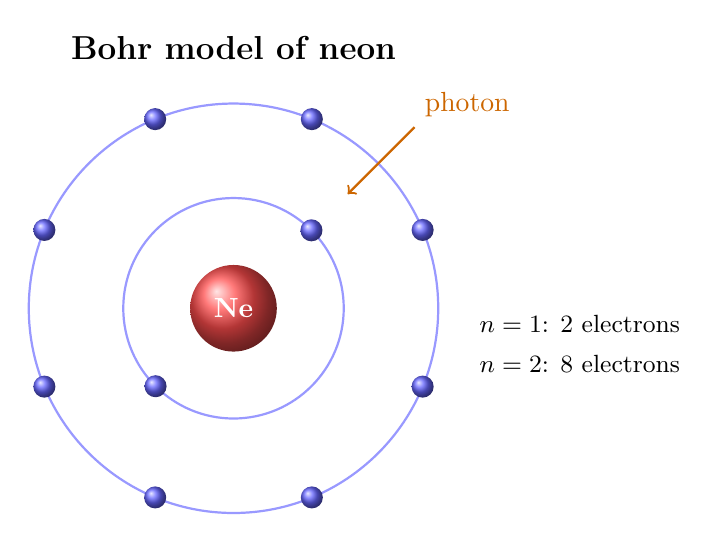
\begin{tikzpicture}
  \foreach \r in {1.4,2.6} \draw[blue!40, thick] (0,0) circle (\r);
  \shade[ball color=red!70] (0,0) circle (0.55);
  \node[white, font=\bfseries] at (0,0) {Ne};
  \foreach \a in {45,225} \shade[ball color=blue!60] (\a:1.4) circle (0.14);
  \foreach \a in {0,45,...,315} \shade[ball color=blue!60] (\a+22.5:2.6) circle (0.14);
  \draw[->, thick, orange!80!black] (2.3,2.3) -- (1.45,1.45) node[pos=0, above right] {photon};
  \node[font=\small, anchor=west] at (3.0,-0.2) {$n=1$: 2 electrons};
  \node[font=\small, anchor=west] at (3.0,-0.7) {$n=2$: 8 electrons};
  \node[font=\large\bfseries] at (0,3.3) {Bohr model of neon};
\end{tikzpicture}
